% !TeX encoding = UTF-8

% 载入 SJTUThesis 模版
\documentclass[type=master]{sjtuthesis}
% 选项
%   type=[doctor|master|bachelor],     % 可选(默认:master),论文类型
%   zihao=[-4|5],                      % 可选(默认:-4),正文字号大小
%   lang=[zh|en|de|ja],                % 可选(默认:zh),论文的主要语言
%   review,                            % 可选(默认:关闭),盲审模式
%   [twoside|oneside],                 % 可选(默认:twoside),双页或单页边距模式
%   [openright|openany],               % 可选(默认:openright),奇数页或任意页开始新章
%   math-style=[ISO|TeX],              % 可选 (默认:ISO),数学符号样式

% 论文基本配置,加载宏包等全局配置
% !TEX root = ./main.tex

\sjtusetup{
  %
  %******************************
  % 注意:
  %   1. 配置里面不要出现空行
  %   2. 不需要的配置信息可以删除
  %******************************
  %
  % 信息录入
  %
  info = {%
    %
    % 标题
    %
    zh / title           = {基于面部捕捉、语音、头部运动的在线实时数字人驱动},
    en / title           = {FaceCapGes: Real-Time Frame-by-Frame Gesture Generation from Audio, Facial Capture, and Head Pose},
    %
    % 标题页标题
    %   可使用“\\”命令手动控制换行
    %
    % zh / display-title   = {上海交通大学学位论文\\ \LaTeX{} 模板示例文档},
    % en / display-title   = {A Sample Document \\ for \LaTeX-based SJTU Thesis Template},
    %
    % 关键词
    %
    zh / keywords        = {协同语音手势生成, 数字人驱动, 面部捕捉, 多模态学习},
    en / keywords        = {co-speech gesture generation, virtual avatar driving, face-capture, multimodal learning},
    %
    % 姓名
    %
    zh / author          = {花泉\quad{}润},
    en / author          = {Jun Hanaizumi},
    %
    % 指导教师
    %
    zh / supervisor      = {杨旭波教授},
    en / supervisor      = {Prof. Xubo Yang},
    %
    % 副指导教师
    %
    % assoc-supervisor  = {某某教授},
    % assoc-supervisor* = {Prof. Uom Uom},
    %
    % 学号
    %
    id              = {122037990002},
    %
    % 学位
    %   本科生不需要填写
    %
    zh / degree          = {工学硕士},
    en / degree          = {Master of Engineering},
    %
    % 专业
    %
    zh / major           = {专业},
    en / major           = {A Very Important Major},
    %
    % 所属院系
    %
    zh / department      = {计算机学院},
    en / department      = {Depart of XXX},
    %
    % 答辩日期
    %   使用 ISO 格式 (yyyy-mm-dd);默认为当前时间
    %
    % date                 = {2023-05-18},
    %
    % 标题页显示日期
    %   覆盖对应标题页的日期显示,原样输出
    %
    % zh / display-date    = {2023 年 5 月},
    %
    % 资助基金
    %
    % zh / fund  = {
    %                {国家 973 项目 (No. 2025CB000000)},
    %                {国家自然科学基金 (No. 81120250000)},
    %              },
    % en / fund  = {
    %                {National Basic Research Program of China (Grant No. 2025CB000000)},
    %                {National Natural Science Foundation of China (Grant No. 81120250000)},
    %              },
  },
  %
  % 风格设置
  %
  style = {%
    %
    % 论文标题页 logo 颜色 (red/blue/black)
    %
    % title-logo-color = black,
  },
  %
  % 名称设置
  %
  name = {
    % bib             = {References},
    % ack             = {谢\hspace{\ccwd}辞},
    % achv            = {攻读学位期间完成的论文},
  },
}

\usepackage{nomencl}

% 使用 BibLaTeX 处理参考文献
%   biblatex-gb7714-2015 常用选项
%     gbnamefmt=lowercase     姓名大小写由输入信息确定
%     gbpub=false             禁用出版信息缺失处理
\usepackage[backend=biber,style=gb7714-2015]{biblatex}
% 文献表字体
% \renewcommand{\bibfont}{\zihao{5}\fixedlineskip{15.6bp}}
% 文献表条目间的间距
\setlength{\bibitemsep}{0pt}
% 导入参考文献数据库
\addbibresource{refs.bib}
% 脚注格式
\usepackage[perpage,bottom,hang]{footmisc}

% 定义图片文件目录与扩展名
\graphicspath{{figures/}}
\DeclareGraphicsExtensions{.pdf,.eps,.png,.jpg,.jpeg}

% 确定浮动对象的位置,可以使用 [H],强制将浮动对象放到这里(可能效果很差)
% \usepackage{float}

% 固定宽度的表格
% \usepackage{tabularx}

% 使用三线表:toprule,midrule,bottomrule。
\usepackage{booktabs}

% 表格中支持跨行
\usepackage{multirow}

% 表格中数字按小数点对齐
\usepackage{dcolumn}
\newcolumntype{d}[1]{D{.}{.}{#1}}

% 使用长表格
\usepackage{longtable}

% 附带脚注的表格
\usepackage{threeparttable}

% 附带脚注的长表格
\usepackage{threeparttablex}

% 算法环境宏包
\usepackage[ruled,vlined,linesnumbered]{algorithm2e}
% \usepackage{algorithm, algorithmicx, algpseudocode}

% 代码环境宏包
\usepackage{listings}
\lstdefinestyle{lstStyleCode}{%
  aboveskip         = \medskipamount,
  belowskip         = \medskipamount,
  basicstyle        = \ttfamily\zihao{6},
  commentstyle      = \slshape\color{black!60},
  stringstyle       = \color{green!40!black!100},
  keywordstyle      = \bfseries\color{blue!50!black},
  extendedchars     = false,
  upquote           = true,
  tabsize           = 2,
  showstringspaces  = false,
  xleftmargin       = 1em,
  xrightmargin      = 1em,
  breaklines        = false,
  framexleftmargin  = 1em,
  framexrightmargin = 1em,
  backgroundcolor   = \color{gray!10},
  columns           = flexible,
  keepspaces        = true,
  texcl             = true,
  mathescape        = true
}
\lstnewenvironment{codeblock}[1][]{%
  \lstset{style=lstStyleCode,#1}}{}

% 直立体数学符号
\providecommand{\dd}{\mathop{}\!\mathrm{d}}
\providecommand{\ee}{\mathrm{e}}
\providecommand{\ii}{\mathrm{i}}
\providecommand{\jj}{\mathrm{j}}

% 国际单位制宏包
\usepackage{siunitx}

% 定理环境宏包
\usepackage{ntheorem}
% \usepackage{amsthm}

% 绘图宏包
\usepackage{tikz}
\usetikzlibrary{arrows.meta, shapes.geometric}

% 一些文档中用到的 logo
\usepackage{hologo}
\providecommand{\XeTeX}{\hologo{XeTeX}}
\providecommand{\BibLaTeX}{\textsc{Bib}\LaTeX}

% 借用 ltxdoc 里面的几个命令方便写文档
\DeclareRobustCommand\cs[1]{\texttt{\char`\\#1}}
\providecommand\pkg[1]{{\sffamily#1}}

% hyperref 宏包在最后调用
\usepackage{hyperref}

% E-mail
\providecommand{\email}[1]{\href{mailto:#1}{\urlstyle{tt}\nolinkurl{#1}}}


\begin{document}

%TC:ignore

% 标题页
\maketitle

% 原创性声明及使用授权书
\copyrightpage
% 插入外置原创性声明及使用授权书
% 此时必须在导言区使用 \usepackage{pdfpages}
% \copyrightpage[scans/sample-copyright.pdf]

% 前置部分
\frontmatter

% 摘要
% !TEX root = ../main.tex

\begin{abstract}[zh]

手势是交流中重要的细节补充与情感表达载体。随着图像识别技术发展,计算机可通过相机识别用户手势指令,手势输入摆脱了对穿戴式检测设备的依赖。随后,手势与语言的关系被进一步分析,使得计算机能从语音生成手势,这让计算机控制的数字人物可在其发言中融入生动的手势动画,满足人类的交流习惯。

然而,手势动作存在空间与体力消耗需求。作为情感表达工具时,人们需耗费较多精力活动肢体以增强说服力或情感表达效果。近年来元宇宙技术的发展,让人们可操控数字人开展远程交流,但受当前技术限制,该场景下的手势生成需依赖穿戴式检测设备,这使得用户在虚拟世界的手势表达较为繁琐。

当前协同语音手势生成技术以获取完整文本为前提,通过语义分析高精度生成对应手势。但对于逐字输入的用户语音,该方式难以提供在线实时的解决方案。考虑到面向用户的应用场景,可同时利用麦克风与相机获取面部表情、头部旋转等其他信息,提供多角度的分析辅助。面部表情可辅助补充文本的情感信息,头部旋转能为手势生成提供朝向指导。这两种信息随语音自然产生,用户负担远低于实际做手势。此外,面部表情与头部旋转的实时获取技术已较为成熟,且具备良好的实时运行性能。

因此,本论文提出 FaceCapGes 方法,基于语音、面部表情、头部旋转三种实时信息,生成在线实时的 3D 手势骨骼动画。该方法可给用户的实时数字形象添加手势动画,无需用户实际做出手势动作。且模型不依赖用户的未来输入,能在实时环境中丰富用户虚拟形象的表达能力。

以往研究已对面部表情、语音与手势的关系进行分析,并提出成熟的学习方法。本模型在现有级联架构基础上,增加头部姿态特征分析模块,同时引入滑动窗口机制以实现架构的实时运行。本模型所依赖的框架及额外添加模块性能开销低,与面部捕捉和头部姿态计算任务同时运行时,仍具备良好的实时性能。

主观评价结果表明,在自然性方面,本方法与当前主流方法相当;在响应速度上,具有显著优势。生成的手势与语音高度对齐,且具备良好的实时交互表现。此外,本模型可部署在 iPhone 等轻量设备上,只要输入格式兼容 ARKit 面部捕捉标准,就能广泛应用于各类实时互动场景。

\end{abstract}

\begin{abstract}[en]

Gesture is an important carrier for supplementary details and emotional expression in communication. With the development of image recognition technology, computers can recognize users' gesture commands through cameras, freeing gesture input from the dependence on wearable detection devices. Subsequently, the relationship between gestures and language has been further analyzed, enabling computers to generate gestures from speech. This allows computer - controlled digital characters to incorporate vivid gesture animations into their speeches, meeting human communication habits.

However, gesture movements have spatial and physical energy consumption requirements. When used as an emotional expression tool, people need to spend a lot of energy moving their limbs to enhance persuasion or emotional expression effects. In recent years, the development of meta - universe technology has allowed people to control digital humans for remote communication. But due to current technical limitations, gesture generation in this scenario needs to rely on wearable detection devices, which makes gesture expression in the virtual world rather cumbersome for users.

The current collaborative speech - gesture generation technology takes the acquisition of complete text as a prerequisite and generates corresponding gestures with high precision through semantic analysis. However, for user speech input word by word, this method is difficult to provide an online real - time solution. Considering the application scenarios for users, other information such as facial expressions and head rotation can be acquired by using microphones and cameras at the same time to provide multi - angle analysis assistance. Facial expressions can assist in supplementing the emotional information of text, and head rotation can provide orientation guidance for gesture generation. These two kinds of information are naturally generated along with speech, and the burden on users is much lower than that of actually making gestures. In addition, the real - time acquisition technology for facial expressions and head rotation is quite mature and has good real - time operation performance.

Therefore, this paper proposes the FaceCapGes method, which generates online real - time 3D gesture skeleton animations based on three kinds of real - time information: speech, facial expressions, and head rotation. This method can add gesture animations to users' real - time digital images without users actually making gesture movements. Moreover, the model does not rely on users' future input and can enrich the expressive ability of users' virtual images in real - time environments.

Previous studies have analyzed the relationships among facial expressions, speech, and gestures and proposed mature learning methods. On the basis of the existing cascaded architecture, this model adds a head posture feature analysis module and introduces a sliding window mechanism to realize the real - time operation of the architecture. The framework relied on by this model and the additionally added modules have low performance overhead. When running simultaneously with facial capture and head posture calculation tasks, it still has good real - time performance.

Subjective evaluation results show that in terms of naturalness, this method is comparable to current mainstream methods; in terms of response speed, it has significant advantages. The generated gestures are highly aligned with speech and have good real - time interaction performance. In addition, this model can be deployed on lightweight devices such as iPhones. As long as the input format is compatible with the ARKit facial capture standard, it can be widely applied to various real - time interaction scenarios.

\end{abstract}


% 目录
\tableofcontents
% 插图索引
\listoffigures*
% 表格索引
\listoftables*
% 算法索引
\listofalgorithms*

% 符号对照表
% !TEX root = ../main.tex

%\begin{nomenclature*}
\label{chap:symb}

\begin{longtable}{rl}
  $\epsilon$  & 介电常数  \\  
  $\mu$       & 磁导率    \\
  $\epsilon$  & 介电常数  \\
  $\mu$       & 磁导率    \\
\end{longtable}

%\end{nomenclature*}


%TC:endignore

% 主体部分
\mainmatter

% 正文内容
% !TEX root = ../main.tex

\chapter{引言}

\section{研究背景和意义}

近年来,随着元宇宙、虚拟社交与直播等领域的相关技术日趋成熟,用户已能够使用任意外观的虚拟人作为交互载体,在虚拟空间中与异地用户进行交流。虚拟人 3D 模型的姿态由其内部骨架关节的旋转参数(如欧拉角、四元数等)定义,最终通过蒙皮渲染技术完成可视化。得益于自动骨骼绑定技术,骨骼动画的生成可消除不同 3D 模型间的骨架拓扑差异,实现跨模型复用。

在虚拟人交互中,穿戴式动作捕捉设备是实时驱动手势的传统方案,其可将用户肢体动作实时转换为骨骼动画,提供直观且沉浸的操控体验。尽管其精度较高,但对于大多数用户而言,此类设备存在功能用途单一、硬件成本昂贵、便携性差等问题,限制了使用频率。因此,在当前的元宇宙社交中,仅少数专业用户会使用此类设备,多数普通用户无法在交互中使用手势,导致了用户体验的不一致。

针对普通用户对低门槛虚拟人交互的需求,基于相机的动作捕捉技术\cite{mediapipefacemesh,AppleARKitTrackingGuide}成为主流替代方案。该技术无需额外硬件,仅通过手机、电脑的内置相机(部分依赖深度相机)即可实时捕捉用户动作。但该方案仍存在两种局限:一是需用户面向相机主动做出手势,导致交互过程中难以同步操作键盘、鼠标,且受相机视野范围限制;二是持续手势动作会产生体力消耗,在直播等长时间场景中,用户疲劳问题尤为突出。”

因此,我们提出一种新的需求:用户无需实际执行手势,而是由计算机结合其实时语音、面部表情与头部姿态,自动生成与之语义和情感相匹配的手势动画。该方法旨在降低使用门槛,并解决操作冲突与体力消耗问题。

然而,现有研究尚未提供成熟的解决方案来满足这一需求。当前多数手势生成方法依赖于完整的语音或文本输入,即在获取整个句子的语义信息后方可开始生成,缺乏仅基于历史与当前信息的实时生成研究。此外,从用户环境中可实时获取的模态主要包括语音、面部表情与头部姿态三种。头部姿态对手势的节奏与朝向具有明确的关系,但利用该模态来增强生成手势的自然度的相关研究尚不充分。

为此,本文提出了一种新颖的实时手势生成模型。该模型以帧为单位,输入语音、面部表情与头部姿态数据,并逐帧输出对应的骨骼动画。本文首次在实时手势生成中,将头部姿态作为一种新的模态引入,利用其与自然手势节奏与朝向的高度相关性,结合语音和面部信息共同提升生成动作的自然度。我们采用级联多模态架构与自回归训练来融合这些模态,以学习其联合表征,从而在严格的实时约束下增强手势的表现力。

本文的主要贡献如下:

\begin{enumerate}
\item 提出了 FaceCapGes,一种帧级实时手势生成模型,使用户无需动作捕捉设备或实际做出手势,仅通过语音等常见输入即可驱动虚拟人的手势动画;
\item 将头部姿态作为新模态引入多模态级联架构,在实时生成约束下有效提升了手势的自然性与表现力;
\item 通过实验结果表明,该模型在手势自然性、语音-手势对齐度与实时响应方面展示了良好的性能。其框架适用于所有兼容 ARKit 的设备。
\end{enumerate}

\section{研究内容}

本文的研究目标是构建一种基于语音、面部捕捉与头部姿态的实时数字人手势生成模型,实现无需动作捕捉设备即可驱动虚拟角色自然表达的实时动画系统。该研究旨在解决现有手势生成方法对未来上下文的依赖及实时性不足的问题,从而为虚拟人交互提供更低门槛、更高沉浸度的解决方案。

为实现上述目标,本文的主要研究内容如下:

其一,设计一种帧级手势生成架构。
为实现帧级实时推理,本架构在基线模型 \cite {beatcamn} 的基础上做两种调整:一方面,保留其语音、面部表情等可实时获取的输入模态,移除非实时模态的输入分支与特征处理模块;另一方面,采用滑动窗口式自回归训练方式,确保模型仅依赖历史与当前帧信息进行推理(不依赖未来上下文),同时通过窗口内时序依赖建模保持动作的时间连续性。由此使架构可处理逐帧输入的实时流数据。

其二,提出一种引入头部姿态的新型模态融合策略。
在现有语音、面部表情生成手势的模型基础上,将头部姿态作为终端模态引入,设计头部姿态编码器并提取特征,以增强生成手势的朝向的自然性。

其三,搭建实验系统与用户测试环境。
本文基于主流渲染引擎构建了虚拟人驱动与手势动画的可视化系统。该系统作为评估平台,为后续的主观实验提供了统一环境。

综上所述,本文引入头部姿态的新模态,来辅助手势生成模型从历史与现在信息推理手势的能力,并且提供了一个实验场景验证模型的推理质量与实时性能。

\section{论文组织架构}

本文共分为六个章节,内容安排如下:

第一章为绪论,介绍本研究的背景与意义,阐述研究目标、主要内容及核心贡献,并说明论文的整体组织结构。

第二章为相关工作, 回顾了国内外在语音驱动手势生成、多模态学习及实时面部捕捉技术等方面的研究现状,分析了现有方法的不足,并明确了本文的研究定位与创新点。

第三章为方法, 详细介绍了本文提出的 FaceCapGes 模型的整体架构与算法流程,包括多模态输入编码、姿态解码机制、滑动窗口自回归训练策略及对抗优化过程。

第四章为评估, 阐述了模型在 BEAT 数据集上的实验设置与性能评估,涵盖客观指标、用户主观实验及消融研究;同时分析了模型在实时交互场景中的表现与应用潜力。

第五章为结论, 总结了本文的主要研究成果与贡献,讨论了当前系统的局限性,并对未来在语义手势生成与跨平台实时驱动方向上的研究进行了展望。

第六章为附录与致谢部分, 包含用户实验的平衡拉丁方设计、附加实验结果、参考文献及致谢内容。

%近年来,已提出多种手势生成方法,包括多层感知机(MLP)\cite{gesticulator2020,beatcamn}、循环神经网络(RNN)\cite{beatcamn}、图神经网络\cite{gesturemaster2022}、扩散模型\cite{diffsheg,diffgesture,DiffTED2024}、VQ-VAE\cite{emage}以及自监督学习方法\cite{diffusion-self-supervised2023}。这些模型在生成质量上表现优异,但大多数依赖离线处理或未来上下文信息,难以满足实时应用需求。部分在线模型已被提出\cite{towards_realtime_co_speech_gesture_generation,realtime_gesture_animation_generation},但往往仍需短时未来窗口,并忽略了常见设备中可用的重要模态信息。

%为解决上述问题,本文提出FaceCapGes,一种无需动作捕捉设备即可实现用户驱动的虚拟人控制的帧级实时手势生成模型。本模型支持在无未来上下文的情况下进行在线推理,能从实时输入中持续预测手势。我们首次引入“头部姿态”作为新模态,与语音和面部捕捉结合,利用其与自然手势节奏的高度相关性,提升生成动作的自然度。各模态通过级联多模态架构进行处理,以学习其联合关系,从而在实时约束下提升手势表达力。

%本方法可部署于轻量设备,具体实现基于配备 Apple ARKit 面部捕捉系统的 iPhone。尽管模型本身计算效率高,具备实时推理能力,但目前仍依赖 BEAT 数据集提供的 ARKit 专用面部数据格式,从中提取面部表情与头部动作。因此,跨平台部署能力仍受限,对通用摄像头、桌面环境或 VR 头显的支持仍是一个开放问题。

%通过在 BEAT 数据集上的实验表明,引入头部姿态显著提升了手势自然性,同时保持了低延迟的实时性能。实验结果说明,即使在无动作捕捉设备与未来输入的情况下,用户也可仅通过语音与头部动作驱动富有表现力的虚拟角色,只要输入符合 ARKit 格式即可。
%为实现实时推理,模型采用滑动窗口的自回归训练策略,并在不依赖未来信息的情况下处理各输入模态。此外,我们使用六维连续旋转表示(Rot6d)\cite{rot6d} 替代传统的欧拉角表示,从而提升动作多样性。后续章节将详细介绍模型架构、训练策略及在 BEAT 数据集上的评估结果,并在主观质量、时序对齐与推理延迟方面与现有手势生成模型进行对比(见图~\ref{fig3},表~\ref{tab1},表~\ref{tab3})。

% !TEX root = ../main.tex

\chapter{数学与引用文献的标注}

\section{数学}

\subsection{数字和单位}

宏包 \pkg{siunitx} 提供了更好的数字和单位支持:
\begin{itemize}
  \item \num{12345.67890}
  \item \complexnum{1+-2i}
  \item \num{.3e45}
  \item \numproduct{1.654 x 2.34 x 3.430}
  \item \unit{kg.m.s^{-1}}
  \item \unit{\micro\meter} $\unit{\micro\meter}$
  \item \unit{\ohm} $\unit{\ohm}$
  \item \numlist{10;20}
  \item \numlist{10;20;30}
  \item \qtylist{0.13;0.67;0.80}{\milli\metre}
  \item \numrange{10}{20}
  \item \qtyrange{10}{20}{\degreeCelsius}
\end{itemize}

\subsection{数学符号和公式}

按照国标 GB/T 3102.11—1993《物理科学和技术中使用的数学符号》,
微分符号 $\dd$ 应使用直立体。除此之外,数学常数也应使用直立体:
\begin{itemize}
  \item 微分符号 $\dd$:\cs{dd}
  \item 圆周率 $\uppi$:\cs{uppi}
  \item 自然对数的底 $\ee$:\cs{ee}
  \item 虚数单位 $\ii$, $\jj$:\cs{ii} \cs{jj}
\end{itemize}

公式应另起一行居中排版。公式后应注明编号,按章顺序编排,编号右端对齐。
\begin{equation}
  \ee^{\ii\uppi} + 1 = 0,
\end{equation}
\begin{equation}
  \frac{\dd^2 u}{\dd t^2} = \int f(x) \dd x.
\end{equation}

公式末尾是需要添加标点符号的,至于用逗号还是句号,取决于公式下面一句是接着公式说的,还是另起一句。
\begin{equation}
  \frac{2h}{\pi}\int_{0}^{\infty}\frac{\sin\left( \omega\delta \right)}{\omega}
  \cos\left( \omega x \right) \dd\omega = 
  \begin{cases}
    h, & \left| x \right| < \delta, \\
    \frac{h}{2}, & x = \pm \delta, \\
    0, & \left| x \right| > \delta.
  \end{cases}
\end{equation}
公式较长时最好在等号“$=$”处转行。
\begin{align}
    & I (X_3; X_4) - I (X_3; X_4 \mid X_1) - I (X_3; X_4 \mid X_2) \nonumber \\
  = & [I (X_3; X_4) - I (X_3; X_4 \mid X_1)] - I (X_3; X_4 \mid \tilde{X}_2) \\
  = & I (X_1; X_3; X_4) - I (X_3; X_4 \mid \tilde{X}_2).
\end{align}

如果在等号处转行难以实现,也可在 $+$、$-$、$\times$、$\div$ 运算符号处转行,转行
时运算符号仅书写于转行式前,不重复书写。
\begin{multline}
  \frac{1}{2} \Delta (f_{ij} f^{ij}) =
    2 \left(\sum_{i<j} \chi_{ij}(\sigma_{i} - \sigma_{j})^{2}
    + f^{ij} \nabla_{j} \nabla_{i} (\Delta f) \right. \\
  \left. + \nabla_{k} f_{ij} \nabla^{k} f^{ij} +
    f^{ij} f^{k} \left[2\nabla_{i}R_{jk}
    - \nabla_{k} R_{ij} \right] \vphantom{\sum_{i<j}} \right).
\end{multline}

\subsection{定理环境}

示例文件中使用 \pkg{ntheorem} 宏包配置了定理、引理和证明等环境。用户也可以使用
\pkg{amsthm} 宏包。

这里举一个“定理”和“证明”的例子。
\begin{theorem}[留数定理]
\label{thm:res}
  假设 $U$ 是复平面上的一个单连通开子集,$a_1, \ldots, a_n$ 是复平面上有限个点,
  $f$ 是定义在 $U \backslash \{a_1, \ldots, a_n\}$ 上的全纯函数,如果 $\gamma$
  是一条把 $a_1, \ldots, a_n$ 包围起来的可求长曲线,但不经过任何一个 $a_k$,并且
  其起点与终点重合,那么:

  \begin{equation}
    \label{eq:res}
    \oint\limits_\gamma f(z)\, \dd z = 2\uppi \ii \sum_{k=1}^n \operatorname{I}(\gamma, a_k) \operatorname{Res}(f, a_k).
  \end{equation}

  如果 $\gamma$ 是若尔当曲线,那么 $\operatorname{I}(\gamma, a_k) = 1$,因此:

  \begin{equation}
    \label{eq:resthm}
    \oint\limits_\gamma f(z)\, \dd z = 2\uppi \ii \sum_{k=1}^n \operatorname{Res}(f, a_k).
  \end{equation}

  在这里,$\operatorname{Res}(f, a_k)$ 表示 $f$ 在点 $a_k$ 的留数,
  $\operatorname{I}(\gamma, a_k)$ 表示 $\gamma$ 关于点 $a_k$ 的卷绕数。卷绕数是
  一个整数,它描述了曲线 $\gamma$ 绕过点 $a_k$ 的次数。如果 $\gamma$ 依逆时针方
  向绕着 $a_k$ 移动,卷绕数就是一个正数,如果 $\gamma$ 根本不绕过 $a_k$,卷绕数
  就是零。

  定理~\ref{thm:res} 的证明。

  \begin{proof}
    首先,由……

    其次,……

    所以……
  \end{proof}
\end{theorem}

\section{引用文献的标注}

按照教务处的要求,参考文献外观应符合国标 GB/T 7714 的要求。模版使用 \BibLaTeX{}
配合 \pkg{biblatex-gb7714-2015} 样式包%
\footnote{\url{https://www.ctan.org/pkg/biblatex-gb7714-2015}}%
控制参考文献的输出样式,后端采用 \pkg{biber} 管理文献。

请注意 \pkg{biblatex-gb7714-2015} 宏包 2016 年 9 月才加入 CTAN,如果你使用的
\TeX{} 系统版本较旧,可能没有包含 \pkg{biblatex-gb7714-2015} 宏包,需要手动安装。
\BibLaTeX{} 与 \pkg{biblatex-gb7714-2015} 目前在活跃地更新,为避免一些兼容性问
题,推荐使用较新的版本。

正文中引用参考文献时,使用 \verb|\cite{key1,key2,key3...}| 可以产生“上标引用的参
考文献”,如 \cite{Yu2001,Cheng1999,LSC1957}。使用
\verb|\parencite{key1,key2,key3...}| 则可以产生水平引用的参考文献,例如
\parencite{Li1999,Jiang1989,Hopkinson1999}。请看下面的例子,将会穿插使用水平的和
上标的参考文献:普通图书\parencite{Yu2001,Jiang1998},论文集、会议录
\cite{CSTAM1990},科技报告\parencite{WHO1970},学位论文\cite{Zhang1998},专利文
献\parencite{Jiang1989,HBLZ2001},专著中析出的文献\cite{Cheng1999,GBT2659},期刊
中析出的文献\parencite{Li1999,Li2000},报纸中析出的文献\cite{Ding2000}, 电子文献
\parencite{Jiang1999,Christine1998,Xiao2001}。

可以使用 \verb|\nocite{key1,key2,key3...}| 将参考文献条目加入到文献表中但不在正
文中引用。使用 \verb|\nocite{*}| 可以将参考文献数据库中的所有条目加入到文献表
中。
\nocite{Yang1999,Schinstock2000,Wen1990,GBT16159}

% !TeX root = ../main.tex

\chapter{浮动体}

\section{插图}

插图功能是利用 \TeX{} 的特定编译程序提供的机制实现的,不同的编译程序支持不同的图
形方式。有的同学可能听说“\LaTeX{} 只支持 EPS”,事实上这种说法是不准确的。\XeTeX{}
可以很方便地插入 EPS、PDF、PNG、JPEG 格式的图片。

一般图形都是处在浮动环境中。之所以称为浮动是指最终排版效果图形的位置不一定与源文
件中的位置对应,这也是刚使用 \LaTeX{} 同学可能遇到的问题。如果要强制固定浮动图形
的位置,请使用 \pkg{float} 宏包,它提供了 \texttt{[H]} 参数。

\subsection{单个图形}

图要有图题,研究生图题采用中英文对照,并置于图的编号之后,图的编号和图题应置于图
下方的居中位置。引用图应在图题右上角标出文献来源。当插图中组成部件由数字或字母等
编号表示时,可在插图下方添加图注进行说明,如图~\ref{fig:cn_100t} 所示。

\begin{figure}[!htp]
  \centering
  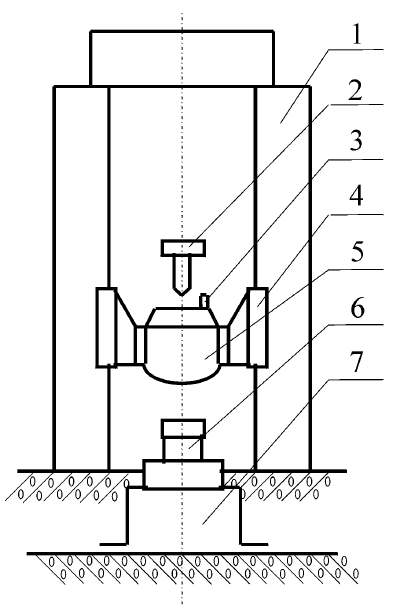
\includegraphics[width=4cm]{cn_100t.png} \\
    1.立柱 2.提升释放机构 3.标准冲击加速度计 \\
    4.导轨 5.重锤 6.被校力传感器 7.底座 \\
  \bicaption[出现在插图索引中]
    {单个图形示例\cite{He1999}。如果表格的标题很长,那么在表格索引中就会很不美观。可
      以在前面用中括号写一个简短的标题,这个标题会出现在索引中。}
    {Stay hungry, stay foolish.}
  \label{fig:cn_100t}
\end{figure}

\subsection{多个图形}

简单插入多个图形的例子如图~\ref{fig:SRR} 所示。这两个水平并列放置的子图共用一个
图形计数器,没有各自的子图题。


\begin{figure}[!htp]
  \centering
  
\includegraphics[height=2cm]{sjtu-vi-badge-blue.pdf}
  \hspace{1cm}
  
\includegraphics[height=2cm]{sjtu-vi-badge-blue.pdf}
  \bicaption{中文题图}{English caption}
  \label{fig:SRR}
\end{figure}

如果多个图形相互独立,并不共用一个图形计数器,那么用 \texttt{minipage} 或者
\texttt{parbox} 就可以,如图~\ref{fig:parallel1} 与图~\ref{fig:parallel2}。

\begin{figure}[!htp]
  \centering
  \begin{minipage}{0.48\textwidth}
    \centering
    
\includegraphics[height=1.5cm]{sjtu-vi-name-blue.pdf}
    \caption{并排第一个图}
    \label{fig:parallel1}
  \end{minipage}\hfill
  \begin{minipage}{0.48\textwidth}
    \centering
    
\includegraphics[height=1.5cm]{sjtu-vi-name-blue.pdf}
    \caption{并排第二个图}
    \label{fig:parallel2}
  \end{minipage}
\end{figure}

如果要为共用一个计数器的多个子图添加子图题,建议使用较新的 \pkg{subcaption}宏
包,不建议使用 \pkg{subfigure} 或 \pkg{subfig} 等宏包。

推荐使用 \pkg{subcaption} 宏包的 \cs{subcaptionbox} 并排子图,子图题置于子图之
下,子图号用 a)、b) 等表示。也可以使用 \pkg{subcaption} 宏包的 \cs{subcaption}
(放在 minipage中,用法同 \cs{caption})。

\pkg{subcaption} 宏包也提供了 \pkg{subfigure} 和 \pkg{subtable} 环境,如
图~\ref{fig:subfigure}。

\begin{figure}[!htp]
  \centering
  \begin{subfigure}{0.3\textwidth}
    \centering
    
\includegraphics[height=2cm]{sjtu-vi-badge-blue.pdf}
    \caption{校徽}
  \end{subfigure}
  \hspace{1cm}
  \begin{subfigure}{0.4\textwidth}
    \centering
    
\includegraphics[height=1.5cm]{sjtu-vi-name-blue.pdf}
    \caption{校名。注意这个图略矮些,subfigure 中同一行的子图在顶端对齐。}
  \end{subfigure}
  \caption{包含子图题的范例(使用 subfigure)}
  \label{fig:subfigure}
\end{figure}

搭配 \pkg{bicaption} 宏包时,可以启用 \cs{subcaptionbox} 和 \cs{subcaption} 的双
语变种 \cs{bisubcaptionbox} 和 \cs{bisubcaption},如图~\ref{fig:bisubcaptionbox}
所示。

\begin{figure}[!hbtp]
  \centering
  \bisubcaptionbox{$R_3 = 1.5\text{mm}$ 时轴承的压力分布云图}%
                  {Pressure contour of bearing when $R_3 = 1.5\text{mm}$}%
                  [6.4cm]{\includegraphics[height=3cm]{example-image-a.pdf}}
  \hspace{1cm}
  \bisubcaptionbox{$R_3 = 2.5\text{mm}$ 时轴承的压力分布云图}%
                  {Pressure contour of bearing when $R_3 = 2.5\text{mm}$}%
                  [6.4cm]{\includegraphics[height=3cm]{example-image-b.pdf}}
  \bicaption{包含子图题的范例(使用 subcaptionbox)}
            {Example with subcaptionbox}
  \label{fig:bisubcaptionbox}
\end{figure}


\section{表格}

\subsection{基本表格}

编排表格应简单明了,表达一致,明晰易懂,表文呼应、内容一致。表题置于表上,研究生
学位论文可以用中、英文两种文字居中排写,中文在上,也可以只用中文。

表格的编排建议采用国际通行的三线表\footnote{三线表,以其形式简洁、功能分明、阅读
方便而在科技论文中被推荐使用。三线表通常只有 3 条线,即顶线、底线和栏目线,没有
竖线。}。三线表可以使用 \pkg{booktabs} 提供的 \cs{toprule}、\cs{midrule} 和
\cs{bottomrule}。它们与 \pkg{longtable} 能很好的配合使用。

\begin{table}[!hpt]
  \caption[一个颇为标准的三线表]{一个颇为标准的三线表\footnotemark}
  \label{tab:firstone}
  \centering
  \begin{tabular}{@{}llr@{}} \toprule
    \multicolumn{2}{c}{Item} \\ \cmidrule(r){1-2}
    Animal & Description & Price (\$)\\ \midrule
    Gnat  & per gram  & 13.65 \\
          & each      & 0.01 \\
    Gnu   & stuffed   & 92.50 \\
    Emu   & stuffed   & 33.33 \\
    Armadillo & frozen & 8.99 \\ \bottomrule
  \end{tabular}
\end{table}
\footnotetext{这个例子来自
  \href{https://mirrors.sjtug.sjtu.edu.cn/ctan/macros/latex/contrib/booktabs/booktabs.pdf}%
  {《Publication quality tables in LaTeX》}(\pkg{booktabs} 宏包的文档)。这也是
  一个在表格中使用脚注的例子,请留意与 \pkg{threeparttable} 实现的效果有何不
  同。}

\subsection{复杂表格}

我们经常会在表格下方标注数据来源,或者对表格里面的条目进行解释。可以用
\pkg{threeparttable} 实现带有脚注的表格,如表~\ref{tab:footnote}。

\begin{table}[!htpb]
  \bicaption{一个带有脚注的表格的例子}{A Table with footnotes}
  \label{tab:footnote}
  \centering
  \begin{threeparttable}[b]
     \begin{tabular}{ccd{4}cccc}
      \toprule
      \multirow{2}*{total} & \multicolumn{2}{c}{20\tnote{a}} & \multicolumn{2}{c}{40} & \multicolumn{2}{c}{60} \\
      \cmidrule(lr){2-3}\cmidrule(lr){4-5}\cmidrule(lr){6-7}
      & www & \multicolumn{1}{c}{k} & www & k & www & k \\ % 使用说明符 d 的列会自动进入数学模式,使用 \multicolumn 对文字表头做特殊处理
      \midrule
      & $\underset{(2.12)}{4.22}$ & 120.0140\tnote{b} & 333.15 & 0.0411 & 444.99 & 0.1387 \\
      & 168.6123 & 10.86 & 255.37 & 0.0353 & 376.14 & 0.1058 \\
      & 6.761    & 0.007 & 235.37 & 0.0267 & 348.66 & 0.1010 \\
      \bottomrule
    \end{tabular}
    \begin{tablenotes}
    \item [a] the first note.
    \item [b] the second note.
    \end{tablenotes}
  \end{threeparttable}
\end{table}

如某个表需要转页接排,可以用 \pkg{longtable} 实现。接排时表题省略,表头应重复书
写,并在右上方写“续表 xx”,如表~\ref{tab:performance}。

\begin{ThreePartTable}
  \begin{TableNotes}
    \item[a] 一个脚注
    \item[b] 另一个脚注
  \end{TableNotes}
  \begin{longtable}[c]{c*{6}{r}}
    \bicaption{实验数据}{Experimental data}
    \label{tab:performance} \\
    \toprule
    测试程序 & \multicolumn{1}{c}{正常运行} & \multicolumn{1}{c}{同步}
      & \multicolumn{1}{c}{检查点} & \multicolumn{1}{c}{卷回恢复}
      & \multicolumn{1}{c}{进程迁移} & \multicolumn{1}{c}{检查点} \\
    & \multicolumn{1}{c}{时间 (s)} & \multicolumn{1}{c}{时间 (s)}
      & \multicolumn{1}{c}{时间 (s)} & \multicolumn{1}{c}{时间 (s)}
      & \multicolumn{1}{c}{时间 (s)} &  文件(KB)\\
    \midrule
    \endfirsthead
    \multicolumn{7}{l}{\textbf{续表~\thetable}} \\
    % 英语论文:\multicolumn{7}{r}{\textbf{Table~\thetable~(continued)}} \\
    \toprule
    测试程序 & \multicolumn{1}{c}{正常运行} & \multicolumn{1}{c}{同步}
      & \multicolumn{1}{c}{检查点} & \multicolumn{1}{c}{卷回恢复}
      & \multicolumn{1}{c}{进程迁移} & \multicolumn{1}{c}{检查点} \\
    & \multicolumn{1}{c}{时间 (s)} & \multicolumn{1}{c}{时间 (s)}
      & \multicolumn{1}{c}{时间 (s)} & \multicolumn{1}{c}{时间 (s)}
      & \multicolumn{1}{c}{时间 (s)}&  文件(KB)\\
    \midrule
    \endhead
    \hline
    \multicolumn{7}{r}{续下页}
    \endfoot
    \insertTableNotes
    \endlastfoot
    CG.A.2 & 23.05 & 0.002 & 0.116 & 0.035 & 0.589 & 32491 \\
    CG.A.4 & 15.06 & 0.003 & 0.067 & 0.021 & 0.351 & 18211 \\
    CG.A.8 & 13.38 & 0.004 & 0.072 & 0.023 & 0.210 & 9890 \\
    CG.B.2 & 867.45 & 0.002 & 0.864 & 0.232 & 3.256 & 228562 \\
    CG.B.4 & 501.61 & 0.003 & 0.438 & 0.136 & 2.075 & 123862 \\
    CG.B.8 & 384.65 & 0.004 & 0.457 & 0.108 & 1.235 & 63777 \\
    MG.A.2 & 112.27 & 0.002 & 0.846 & 0.237 & 3.930 & 236473 \\
    MG.A.4 & 59.84 & 0.003 & 0.442 & 0.128 & 2.070 & 123875 \\
    MG.A.8 & 31.38 & 0.003 & 0.476 & 0.114 & 1.041 & 60627 \\
    MG.B.2 & 526.28 & 0.002 & 0.821 & 0.238 & 4.176 & 236635 \\
    MG.B.4 & 280.11 & 0.003 & 0.432 & 0.130 & 1.706 & 123793 \\
    MG.B.8 & 148.29 & 0.003 & 0.442 & 0.116 & 0.893 & 60600 \\
    LU.A.2 & 2116.54 & 0.002 & 0.110 & 0.030 & 0.532 & 28754 \\
    LU.A.4 & 1102.50 & 0.002 & 0.069 & 0.017 & 0.255 & 14915 \\
    LU.A.8 & 574.47 & 0.003 & 0.067 & 0.016 & 0.192 & 8655 \\
    LU.B.2 & 9712.87 & 0.002 & 0.357 & 0.104 & 1.734 & 101975 \\
    LU.B.4 & 4757.80 & 0.003 & 0.190 & 0.056 & 0.808 & 53522 \\
    LU.B.8 & 2444.05 & 0.004 & 0.222 & 0.057 & 0.548 & 30134 \\
    EP.A.2 & 123.81 & 0.002 & 0.010 & 0.003 & 0.074 & 1834 \\
    EP.A.4 & 61.92 & 0.003 & 0.011 & 0.004 & 0.073 & 1743 \\
    EP.A.8 & 31.06 & 0.004 & 0.017 & 0.005 & 0.073 & 1661 \\
    EP.B.2 & 495.49 & 0.001 & 0.009 & 0.003 & 0.196 & 2011 \\
    EP.B.4 & 247.69 & 0.002 & 0.012 & 0.004 & 0.122 & 1663 \\
    EP.B.8 & 126.74 & 0.003 & 0.017 & 0.005 & 0.083 & 1656 \\
    SP.A.2 & 123.81 & 0.002 & 0.010 & 0.003 & 0.074 & 1854 \\
    SP.A.4 & 51.92 & 0.003 & 0.011 & 0.004 & 0.073 & 1543 \\
    SP.A.8 & 31.06 & 0.004 & 0.017 & 0.005 & 0.073 & 1671 \\
    SP.B.2 & 495.49 & 0.001 & 0.009 & 0.003 & 0.196 & 2411 \\
    SP.B.4 \tnote{a} & 247.69 & 0.002 & 0.014 & 0.006 & 0.152 & 2653 \\
    SP.B.8 \tnote{b} & 126.74 & 0.003 & 0.017 & 0.005 & 0.082 & 1755 \\
    \bottomrule
  \end{longtable}
\end{ThreePartTable}

\section{算法环境}

算法环境可以使用 \pkg{algorithms} 宏包或者较新的 \pkg{algorithm2e} 实现。
算法~\ref{algo:algorithm} 是一个使用 \pkg{algorithm2e} 的例子。关于排版算法环境
的具体方法,请阅读相关宏包的官方文档。

\begin{algorithm}[htb]
  \caption{算法示例}
  \label{algo:algorithm}
  \small
  \SetAlgoLined
  \KwData{this text}
  \KwResult{how to write algorithm with \LaTeXe }

  initialization\;
  \While{not at end of this document}{
    read current\;
    \eIf{understand}{
      go to next section\;
      current section becomes this one\;
    }{
      go back to the beginning of current section\;
    }
  }
\end{algorithm}

\section{代码环境}

我们可以在论文中插入算法,但是不建议插入大段的代码。如果确实需要插入代码,建议使
用 \pkg{listings} 宏包。

\begin{codeblock}[language=C]
#include <stdio.h>
#include <unistd.h>
#include <sys/types.h>
#include <sys/wait.h>

int main() {
  pid_t pid;

  switch ((pid = fork())) {
  case -1:
    printf("fork failed\n");
    break;
  case 0:
    /* child calls exec */
    execl("/bin/ls", "ls", "-l", (char*)0);
    printf("execl failed\n");
    break;
  default:
    /* parent uses wait to suspend execution until child finishes */
    wait((int*)0);
    printf("is completed\n");
    break;
  }

  return 0;
}
\end{codeblock}

% !TEX root = ../main.tex

\chapter{全文总结}

这里是全文总结内容。

2015 年 2 月 28 日,中央在北京召开全国精神文明建设工作表彰暨学雷锋志愿服务大会,
公布全国文明城市(区)、文明村镇、文明单位名单。上海交通大学荣获全国文明单位称
号。

全国文明单位这一荣誉是对交大人始终高度重视文明文化工作的肯定,是对交大长期以来文
明创建工作成绩的褒奖。在学校党委、文明委的领导下,交大坚持将文明创建工作纳入学校
建设世界一流大学的工作中,全体师生医护员工群策群力、积极开拓,落实国家和上海市有
关文明创建的各项要求,以改革创新、科学发展为主线,以质量提升为目标,聚焦文明创建
工作出现的重点和难点,优化文明创建工作机制,传播学校良好形象,提升社会美誉度,显
著增强学校软实力。2007 至 2012 年间,上海交大连续三届荣获“上海市文明单位”称
号,成为创建全国文明单位的新起点。

上海交大自启动争创全国文明单位工作以来,凝魂聚气、改革创新,积极培育和践行社会主
义核心价值观。坚持统筹兼顾、多措并举,将争创全国文明单位与学校各项中心工作紧密结
合,着力构建学校文明创建新格局,不断提升师生医护员工文明素养,以“冲击世界一流大
学汇聚强大精神动力”为指导思想,以“聚焦改革、多元推进、以评促建、丰富内涵、彰显
特色”为工作原则,并由全体校领导群策领衔“党的建设深化、思想教育深入、办学成绩显
著、大学文化丰富、校园环境优化、社会责任担当”六大板块共 28 项重点突破工作,全面
展现近年来交大文明创建工作的全貌和成就。

进入新阶段,学校将继续开拓文明创建工作新格局,不断深化工作理念和工作实践,创新工
作载体、丰富活动内涵、凸显创建成效,积极服务于学校各项中心工作和改革发展的大局
面,在上级党委、文明委的关心下,在学校党委的直接领导下,与时俱进、开拓创新,为深
化内涵建设、加快建成世界一流大学、推动国家进步和社会发展而努力奋斗!

上海交通大学医学院附属仁济医院也获得全国文明单位称号。


%TC:ignore

% 参考文献
\printbibliography[heading=bibintoc]

% 附录
\appendix

% 附录中图表不加入索引
\captionsetup{list=no}

% 附录内容
% !TEX root = ../main.tex

\chapter{Maxwell Equations}

选择二维情况,有如下的偏振矢量:
\begin{subequations}
  \begin{align}
    {\bf E} &= E_z(r, \theta) \hat{\bf z}, \\
    {\bf H} &= H_r(r, \theta) \hat{\bf r} + H_\theta(r, \theta) \hat{\bm\theta}.
  \end{align}
\end{subequations}
对上式求旋度:
\begin{subequations}
  \begin{align}
    \nabla \times {\bf E} &= \frac{1}{r} \frac{\partial E_z}{\partial\theta}
      \hat{\bf r} - \frac{\partial E_z}{\partial r} \hat{\bm\theta}, \\
    \nabla \times {\bf H} &= \left[\frac{1}{r} \frac{\partial}{\partial r}
      (r H_\theta) - \frac{1}{r} \frac{\partial H_r}{\partial\theta} \right]
      \hat{\bf z}.
  \end{align}
\end{subequations}
因为在柱坐标系下,$\overline{\overline\mu}$ 是对角的,所以 Maxwell 方程组中电场
$\bf E$ 的旋度:
\begin{subequations}
  \begin{align}
    & \nabla \times {\bf E} = \ii \omega {\bf B}, \\
    & \frac{1}{r} \frac{\partial E_z}{\partial\theta} \hat{\bf r} -
      \frac{\partial E_z}{\partial r}\hat{\bm\theta} = \ii \omega \mu_r H_r
      \hat{\bf r} + \ii \omega \mu_\theta H_\theta \hat{\bm\theta}.
  \end{align}
\end{subequations}
所以 $\bf H$ 的各个分量可以写为:
\begin{subequations}
  \begin{align}
    H_r &= \frac{1}{\ii \omega \mu_r} \frac{1}{r}
      \frac{\partial E_z}{\partial\theta}, \\
    H_\theta &= -\frac{1}{\ii \omega \mu_\theta}
      \frac{\partial E_z}{\partial r}.
  \end{align}
\end{subequations}
同样地,在柱坐标系下,$\overline{\overline\epsilon}$ 是对角的,所以 Maxwell 方程
组中磁场 $\bf H$ 的旋度:
\begin{subequations}
  \begin{align}
    & \nabla \times {\bf H} = -\ii \omega {\bf D}, \\
    & \left[\frac{1}{r} \frac{\partial}{\partial r}(r H_\theta) - \frac{1}{r}
      \frac{\partial H_r}{\partial\theta} \right] \hat{\bf z} = -\ii \omega
      {\overline{\overline\epsilon}} {\bf E} = -\ii \omega \epsilon_z E_z
      \hat{\bf z}, \\
    & \frac{1}{r} \frac{\partial}{\partial r}(r H_\theta) - \frac{1}{r}
      \frac{\partial H_r}{\partial\theta} = -\ii \omega \epsilon_z E_z.
  \end{align}
\end{subequations}
由此我们可以得到关于 $E_z$ 的波函数方程:
\begin{equation}
  \frac{1}{\mu_\theta \epsilon_z} \frac{1}{r} \frac{\partial}{\partial r}
  \left(r \frac{\partial E_z}{\partial r} \right) + \frac{1}{\mu_r \epsilon_z}
  \frac{1}{r^2} \frac{\partial^2E_z}{\partial\theta^2} +\omega^2 E_z = 0.
\end{equation}

% !TEX root = ../main.tex

\chapter{绘制流程图}

图~\ref{fig:flow_chart} 是一张流程图示意。使用 \pkg{tikz} 环境,搭配四种预定义节
点(\verb|startstop|、\verb|process|、\verb|decision| 和 \verb|io|),可以容易地
绘制出流程图。

\begin{figure}[!htp]
  \centering
  
% 定义流程图节点
\tikzstyle{startstop} = [
  rectangle,
  rounded corners,
  minimum width=4em,
  text centered,
  inner sep=1.5ex,
  draw
]
\tikzstyle{io} = [
  trapezium,
  trapezium left angle=75,
  trapezium right angle=105,
  minimum width=4em,
  text centered,
  inner sep=1.5ex,
  draw
]
\tikzstyle{process} = [
  rectangle,
  minimum width=4em,
  text centered,
  inner sep=1.5ex,
  draw
]
\tikzstyle{decision} = [
  diamond,
  minimum width=4em,
  aspect=2,
  text centered,
  draw
]
\tikzstyle{arrow} = [-{LaTeX}]

\begin{tikzpicture}[node distance=1.5cm, every node/.style={font=\footnotesize}]
  % 设置节点
  \node[startstop] (pic) {待测图片};
  \node[io, below of=pic] (bg) {读取背景};
  \node[process, below of=bg] (pair) {匹配特征点对};
  \node[decision, below of=pair, yshift=-2ex] (threshold) {多于阈值};
  \node[decision, right of=threshold, xshift=3cm] (clear) {清晰?};
  \node[process, right of=pair, xshift=3cm] (capture) {重采};
  \node[process, below of=threshold, yshift=-2ex] (matrix_p) {透视变换矩阵};
  \node[process, right of=matrix_p, xshift=3cm] (matrix_a) {仿射变换矩阵};
  \node[process, below of=matrix_p] (reg) {图像修正};
  \node[startstop, below of=reg] (return) {配准结果};
    
  % 连接节点
  \draw[arrow] (pic) -- (bg);
  \draw[arrow] (bg) -- (pair);
  \draw[arrow] (pair) -- (threshold);

  \draw[arrow] (threshold) -- node[above] {否} (clear);

  \draw[arrow] (clear) -- node[right] {否} (capture);
  \draw[arrow] (capture) |- (pic);
  \draw[arrow] (clear) -- node[right] {是} (matrix_a);
  \draw[arrow] (matrix_a) |- (reg);

  \draw[arrow] (threshold) -- node[left] {是} (matrix_p);
  \draw[arrow] (matrix_p) -- (reg);
  \draw[arrow] (reg) -- (return);
\end{tikzpicture}

  \bicaption{绘制流程图效果}{Flow chart}
  \label{fig:flow_chart}
\end{figure}


% 结尾部分
\backmatter

% 用于盲审的论文需隐去致谢、发表论文、科研成果、简历

% 致谢
% !TEX root = ../main.tex

\begin{acknowledgements}
  感谢那位最先制作出博士学位论文 \LaTeX{} 模板的物理系同学!

  感谢 William Wang 同学对模板移植做出的贡献!

  感谢 \href{https://github.com/weijianwen}{@weijianwen} 学长开创性的工作!

  感谢 \href{https://github.com/sjtug}{@sjtug} 对 0.10 及之后版本的开发和维护工作!

  感谢所有为模板贡献过代码的\href{https://github.com/sjtug/SJTUThesis/graphs/contributors}{同学们}, 以及所有测试和使用模板的各位同学!

  感谢 \LaTeX 和 \href{https://github.com/sjtug/SJTUThesis}{SJTUThesis},帮我节省了不少时间。
\end{acknowledgements}


% 发表论文及科研成果
% 盲审论文中,发表论文及科研成果等仅以第几作者注明即可,不要出现作者或他人姓名
% !TEX root = ../main.tex

\begin{achievements}

\subsection*{学术论文}

\begin{bibliolist}{00}
  \item Chen H, Chan C~T. Acoustic cloaking in three dimensions using acoustic metamaterials[J]. Applied Physics Letters, 2007, 91:183518.
  \item Chen H, Wu B~I, Zhang B, et al. Electromagnetic Wave Interactions with a Metamaterial Cloak[J]. Physical Review Letters, 2007, 99(6):63903.
\end{bibliolist}

\begin{bibliolist*}{00}
  \item 第一作者. 中文核心期刊论文, 2007.
  \item 第一作者. EI 国际会议论文, 2006.
\end{bibliolist*}

\subsection*{专利}

\begin{bibliolist}{00}
  \item 第一发明人, “永动机”, 专利申请号202510149890.0.
\end{bibliolist}

\begin{bibliolist*}{00}
  \item 第一发明人, “永动机”, 专利申请号XXXXXXXXXXXX.X.
\end{bibliolist*}

\end{achievements}


% 简历
% !TEX root = ../main.tex

\begin{resume}
  \subsection*{基本情况}
    某某,yyyy 年 mm 月生于 xxxx。

  \subsection*{教育背景}
  \begin{itemize}
    \item yyyy 年 mm 月至今,上海交通大学,博士研究生,xx 专业
    \item yyyy 年 mm 月至 yyyy 年 mm 月,上海交通大学,硕士研究生,xx 专业
    \item yyyy 年 mm 月至 yyyy 年 mm 月,上海交通大学,本科,xx 专业
  \end{itemize}

  \subsection*{研究兴趣}
    \LaTeX{} 排版

  \subsection*{联系方式}
  \begin{itemize}
    \item 地址: 上海市闵行区东川路 800 号,200240
    \item E-mail: \email{john_smith@sjtu.edu.cn}
  \end{itemize}
\end{resume}


% 学士学位论文要求在最后有一个大摘要,单独编页码
% !TEX root = ../main.tex

\begin{digest}
  An imperial edict issued in 1896 by Emperor Guangxu, established Nanyang
  Public School in Shanghai. The normal school, school of foreign studies,
  middle school and a high school were established. Sheng Xuanhuai, the person
  responsible for proposing the idea to the emperor, became the first president
  and is regarded as the founder of the university.

  During the 1930s, the university gained a reputation of nurturing top
  engineers. After the foundation of People's Republic, some faculties were
  transferred to other universities. A significant amount of its faculty were
  sent in 1956, by the national government, to Xi'an to help build up Xi'an Jiao
  Tong University in western China. Afterwards, the school was officially
  renamed Shanghai Jiao Tong University.

  Since the reform and opening up policy in China, SJTU has taken the lead in
  management reform of institutions for higher education, regaining its vigor
  and vitality with an unprecedented momentum of growth. SJTU includes five
  beautiful campuses, Xuhui, Minhang, Luwan Qibao, and Fahua, taking up an area
  of about \qty{3225833}{\square\metre}. A number of disciplines have been
  advancing towards the top echelon internationally, and a batch of burgeoning
  branches of learning have taken an important position domestically.

  Today SJTU has 31 schools (departments), 63 undergraduate programs, 250
  masters-degree programs, 203 Ph.D. programs, 28 post-doctorate programs, and
  11 state key laboratories and national engineering research centers.

  SJTU boasts a large number of famous scientists and professors, including 35
  academics of the Academy of Sciences and Academy of Engineering, 95 accredited
  professors and chair professors of the ``Cheung Kong Scholars Program'' and
  more than \num{2000} professors and associate professors.

  Its total enrollment of students amounts to \num{35929}, of which \num{1564}
  are international students. There are \num{16802} undergraduates, and
  \num{17563} masters and Ph.D. candidates. After more than a century of
  operation, Jiao Tong University has inherited the old tradition of ``high
  starting points, solid foundation, strict requirements and extensive
  practice.'' Students from SJTU have won top prizes in various competitions,
  including ACM International Collegiate Programming Contest, International
  Mathematical Contest in Modeling and Electronics Design Contests. Famous
  alumni include Jiang Zemin, Lu Dingyi, Ding Guangen, Wang Daohan, Qian Xuesen,
  Wu Wenjun, Zou Taofen, Mao Yisheng, Cai Er, Huang Yanpei, Shao Lizi, Wang An
  and many more. More than 200 of the academics of the Chinese Academy of
  Sciences and Chinese Academy of Engineering are alumni of Jiao Tong
  University.
\end{digest}


%TC:endignore

\end{document}
